%% This is file `mcmthesis-demo.tex',
%% generated with the docstrip utility.
%%
%% The original source files were:
%%
%% mcmthesis.dtx  (with options: `demo')
%%
%% -----------------------------------
%%
%% This is a generated file.
%%
%% Copyright (C)
%%       2010 -- 2015 by Zhaoli Wang
%%       2014 -- 2019 by Liam Huang
%%       2019 -- present by latexstudio.net
%%
%% This work may be distributed and/or modified under the
%% conditions of the LaTeX Project Public License, either version 1.3
%% of this license or (at your option) any later version.
%% The latest version of this license is in
%%   http://www.latex-project.org/lppl.txt
%% and version 1.3 or later is part of all distributions of LaTeX
%% version 2005/12/01 or later.
%%
%% This work has the LPPL maintenance status `maintained'.
%%
%% The Current Maintainer of this work is Liam Huang.
%%
%%
%% This is file `mcmthesis-demo.tex',
%% generated with the docstrip utility.
%%
%% The original source files were:
%%
%% mcmthesis.dtx  (with options: `demo')
%%
%% -----------------------------------
%%
%% This is a generated file.
%%
%% Copyright (C)
%%       2010 -- 2015 by Zhaoli Wang
%%       2014 -- 2019 by Liam Huang
%%       2019 -- present by latexstudio.net
%%
%% This work may be distributed and/or modified under the
%% conditions of the LaTeX Project Public License, either version 1.3
%% of this license or (at your option) any later version.
%% The latest version of this license is in
%%   http://www.latex-project.org/lppl.txt
%% and version 1.3 or later is part of all distributions of LaTeX
%% version 2005/12/01 or later.
%%
%% This work has the LPPL maintenance status `maintained'.
%%
%% The Current Maintainer of this work is Liam Huang.
%%
\documentclass{mcmthesis}
\mcmsetup{CTeX = false,    % 使用 CTeX 套装时,设置为 true
          tcn = {Group1},problem = {SET2700G},
          sheet = true, titleinsheet = true, keywordsinsheet = true,
          titlepage = false, abstract = false,author = true}
        
\usepackage{newtxtext}     % \usepackage{palatino}
\usepackage[backend=bibtex]{biblatex}   % for RStudio Complie
\usepackage{biblatex}
\usepackage{tocloft}
\usepackage{subcaption}
\usepackage{lastpage}
\addbibresource{ai.bib} % 添加参考文献文件
\setlength{\cftbeforesecskip}{6pt}
\renewcommand{\contentsname}{\hspace*{\fill}\Large\bfseries Contents \hspace*{\fill}}

\title{Using machine learning methods to identify novel compounds}
\author{Hanmo Shi,Qixuan Wang,Yingying He, Yuxiang Tian} 
% \author{\small \href{http://www.latexstudio.net/}
%   {\includegraphics[width=7cm]{mcmthesis-logo}}}
\date{\today}

\begin{document}
    
\begin{abstract}

    The rising costs and inefficiencies in traditional drug development call for innovative solutions. This study explores the application of artificial intelligence and machine learning to make the drug discovery process more efficient. By integrating semi-supervised and weakly supervised learning approaches with vision-language models, we enhance the analysis and classification of drug compounds. Using data from sources such as PubChem and DrugBank, convolutional neural networks (CNNs) and the VGG-16 architecture are employed to predict pharmaceutical properties and ensure drug safety. The results demonstrate significant improvements in the speed and accuracy of compound screening. Future directions include model optimization, such as pruning and quantization, and incorporating hybrid machine learning techniques to maximize performance while minimizing computational demands.
\begin{keywords}
Machine Learning,Drug Discovery,Convolutional Neural Networks,VGG-16,Data Augmentation
\end{keywords}

\end{abstract}

\maketitle

%% Generate the Table of Contents, if it's needed.
% \renewcommand{\contentsname}{\centering Contents}
\tableofcontents        % 若不想要目录, 注释掉该句
\thispagestyle{empty}
\newpage
\section{Introduction}

\subsection{Background}

Traditional drug development faces significant challenges, including complex reaction pathways, low experimental efficiency, and excessive resource consumption. These issues result in high costs, prolonged development cycles, and limited innovation \cite{atanasov2021natural}. The reliance on trial-and-error methods and manual experimentation further restricts the scalability and speed of drug discovery. Recent advancements in machine learning, particularly in deep learning, offer promising solutions to these challenges. Machine learning can optimize the drug development process, enhance compound identification, accelerate screening, and reduce the need for costly experiments, making it a transformative tool in the field \cite{deng2022artificial}.

\subsection{Our Research Focus}

Our research focuses on leveraging Convolutional Neural Networks (CNNs) to analyze drug compounds using 2D molecular data. CNNs excel in image-based pattern recognition, making them ideal for identifying subtle patterns in complex chemical structures \cite{krizhevsky2012imagenet}. While previous studies have demonstrated the utility of CNNs in analyzing 2D chemical representations, limitations remain, such as the inability to modify 2D structures without altering their chemical meaning \cite{hirohara2018convolutional}. Our work aims to overcome these limitations by applying advanced machine learning techniques to 2D molecular data, ultimately accelerating drug discovery and reducing reliance on traditional trial-and-error methods \cite{park2022brief}. Additionally, we explore the use of hybrid models, such as combining CNNs with transformers, to improve compound-protein interaction predictions \cite{qian2022cat}, and evaluate pre-trained CNN models for 2D image-based drug discovery \cite{banegas2024evaluation}. By leveraging these techniques, we aim to enhance the efficiency and accuracy of drug discovery processes.
\section{Datasets}
\subsection{CID and SMILES}
We first extract CID(Chemical Identifier),a unique numerical identifier assigned to chemical compounds in databases from PubChem. Each CID corresponds to a specific chemical substance, enabling precise referencing, retrieval, and analysis of chemical.Then we can utilize the CIDs we gained to generate SMILES,which was proposed by (\cite{weininger1988smiles}) is currently widely recognized and used as a standard representation of compounds for modern chemical information processing.Then we can gain the classified SMILEs as below.(Table.~\ref{table:medical_terms})

\begin{table}[h!]
\centering
\begin{tabular}{|c|l|p{10cm}|}
\hline
\textbf{Categories} & \textbf{Effect} \\ \hline
Antibacterial & Inhibits or kills bacteria. \\ \hline
Antiviral & Inhibits or kills viruses. \\ \hline
Antifungal & Inhibits or kills fungi. \\ \hline
Antiprotozoal & Inhibits or kills protozoa. \\ \hline
Anti-inflammatory & Relieves or suppresses inflammation. \\ \hline
Antipyretic & Reduces fever and relieves high temperature. \\ \hline
Analgesic & Relieves pain. \\ \hline
Antioxidant & Prevents or reduces oxidative cell damage. \\ \hline
Antitumor & Inhibits the growth and spread of tumors. \\ \hline
Antidepressant & Relieves symptoms of depression. \\ \hline
Sedative & Calms agitation and reduces anxiety. \\ \hline
Hypnotic & Induces sleep and helps with insomnia. \\ \hline
Antihypertensive & Lowers blood pressure. \\ \hline
Antidiabetic & Used to control diabetes. \\ \hline
Antihistamine & Blocks histamine effects, relieves allergies. \\ \hline
Antispasmodic & Relieves muscle spasms or intestinal cramps. \\ \hline
Diuretic & Increases urine output, reduces fluid retention. \\ \hline
\end{tabular}
\caption{Types and effects of drugs in the datasets}
\label{table:medical_terms}
\end{table}
\subsection{Crawl data from websites}
We use the Selenium module to write scripts for crawling CID data from the PubChem website, which contains the information of the CIDs in our datasets. The process is as follows:
\begin{figure}[htbp]
    \centering
    \begin{subfigure}{0.3\textwidth}
        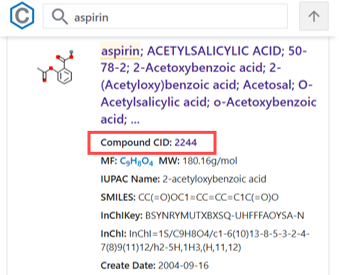
\includegraphics[width=\linewidth]{pics/aspirin_cid.png}
        \caption{Aspirin CID}
        \label{fig:Aspirin CID}
    \end{subfigure}
    \hfill
    \begin{subfigure}{0.3\textwidth}
        
\includegraphics[width=\linewidth]{pics/aspirin_smiles.png}
        \caption{Aspirin SMILES}
        \label{fig:Aspirin SMILES}
    \end{subfigure}
    \hfill
    \begin{subfigure}{0.3\textwidth}
        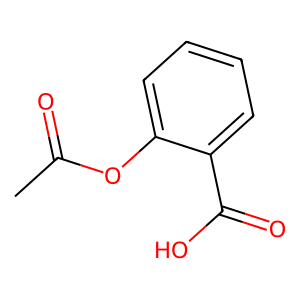
\includegraphics[width=\linewidth]{pics/aspirin_2d.png}
        \caption{Aspirin 2D Image}
        \label{fig:Aspirin 2D Image}
    \end{subfigure}
    \caption{How to get data}
    \label{fig:How to get data}
\end{figure}
\begin{itemize}
    \item Use the Selenium module to write scripts for crawling CID data from the PubChem website(Fig.~\ref{fig:Aspirin CID}).
    \item Translate the CIDs into SMILES format(Fig.~\ref{fig:Aspirin SMILES}), which is the standard representation of chemical compounds.
    \item Further convert the SMILES into 2D(Fig.~\ref{fig:Aspirin 2D Image}) images of the compounds.
\end{itemize}
A detailed demo video can be found in our GitHub repository.
After the work of translation,we would be able to obtain the images of compounds,which would be our datasets.

\section{Traditional CNN}
\subsection{Related Work}
The most important article in the field of CNNs is widely considered to be \cite{krizhevsky2012imagenet}. This paper introduced AlexNet, which won the ImageNet Large Scale Visual Recognition Challenge with a significant margin over traditional machine learning methods.The most important innovation of their work is the introduction of the ReLU Activation and Dropout Regularization.The ReLU Activation is the nonlinearity 
\begin{equation}
    f(x) = max(0,x)
\end{equation}
which could be several times faster than their equivalents with tradition units. Here is the architecture of their CNN.(Fig.~\ref{fig:Traditional_Architecture_of_CNN})

\begin{figure}[htbp]
\centering
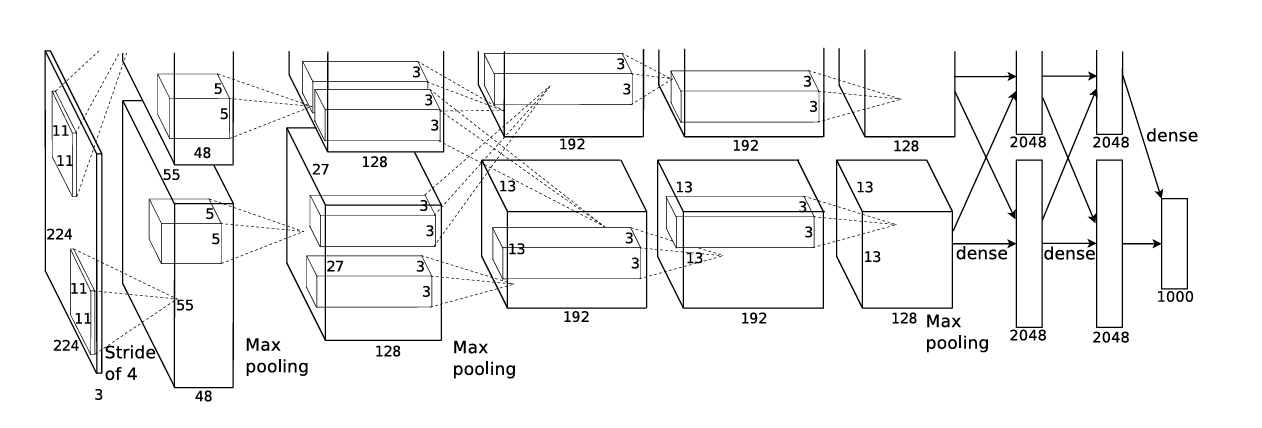
\includegraphics[width = \textwidth]{pics/Traditional_Architecture_of_CNN.png}
\caption{The illustration of the architecture of the original CNN}
\label{fig:Traditional_Architecture_of_CNN}
\end{figure}

\subsection{Our Model}
According to their work,our model(Fig.~\ref{fig:Thumbnails_of_Our_CNN_model}) is organized into three main sections: input layer, feature extraction, and classifier, ending in an output layer. Here’s a detailed breakdown:

\begin{figure}[htbp]
\centering
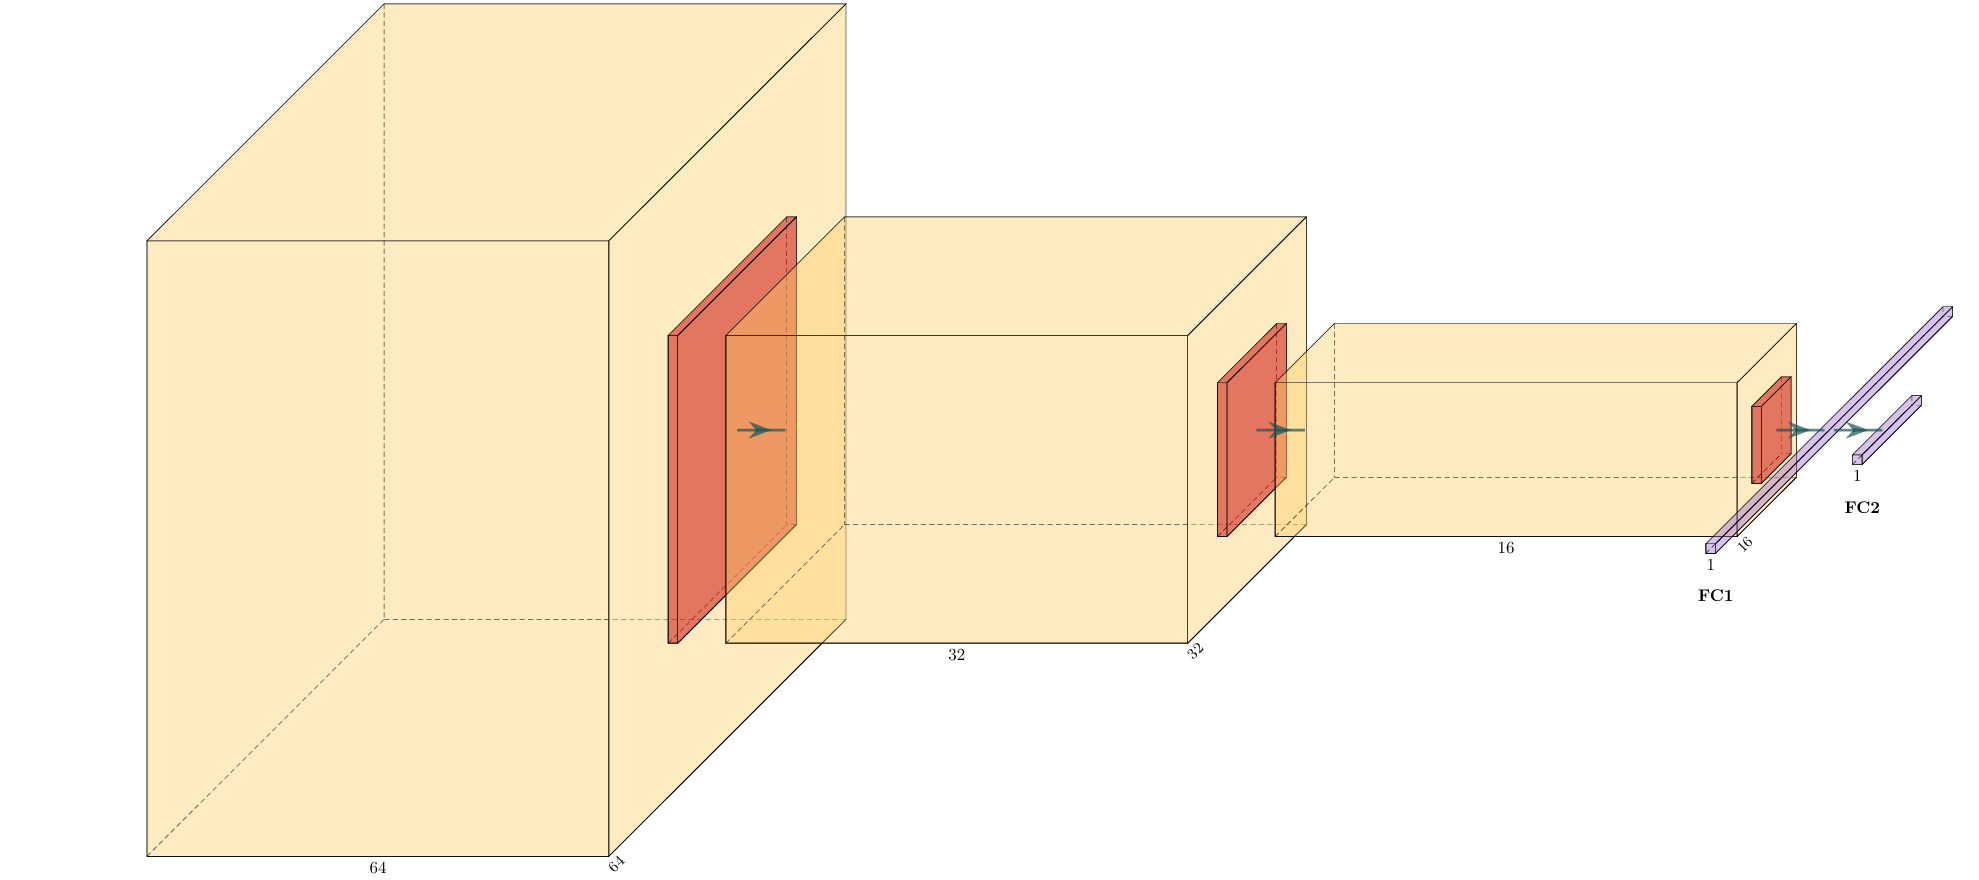
\includegraphics[width =\textwidth]{pics/Thumbnails_of_Our_CNN_model.png}
\caption{Thumbnails of Our CNN Model}
\label{fig:Thumbnails_of_Our_CNN_model}
\end{figure}

(1)Input Layer:The input layer accepts an image of dimensions , where 3 represents the RGB color channels, and H and W are the height and width of the image. (2)Feature Extraction: The feature extraction stage comprises three convolutional blocks.The first Conv2D layer transforms the input using 64 filters of size 3$\times$3 with padding of 1.The output shape is [64,H/2,W/2] , reflecting reduced spatial dimensions due to max-pooling.Another Conv2D layer with 128 filters and a kernel size of 3$\times$3  is applied.As we can see,Max-pooling reduces dimensions further with a kernel size of 2 and stride of 2.
The resulting shape is [128,H/4,W/4] .The last Conv2D layer with 256 filters and a kernel size of 3$\times$3 , followed by ReLU activation.Max-pooling reduces the dimensions again, resulting in an output of shape [256,H/8,W/8] .At last ,after the work of flatten Layer,The 3D output from the feature extraction phase is flattened into a 2D tensor with batch size 256$\times$[H/8]$\times$[W/8]. This operation prepares the data for the fully connected layers in the classifier.
(3)Classifier:The classifier is consisted of two fully connected layers.With the assistance of ReLU activation and dropout,the first layer transfers the flattened input to 1024 neurons and the second transfers the 1024 neurons to the class they belong,which is the output.

\subsection{Result}
Our train loss and train accuracy along with validation accuracy over epochs are as follows.(Fig.~\ref{fig:Train_Loss_and_Accuracy})

\begin{figure}[htbp]
\centering
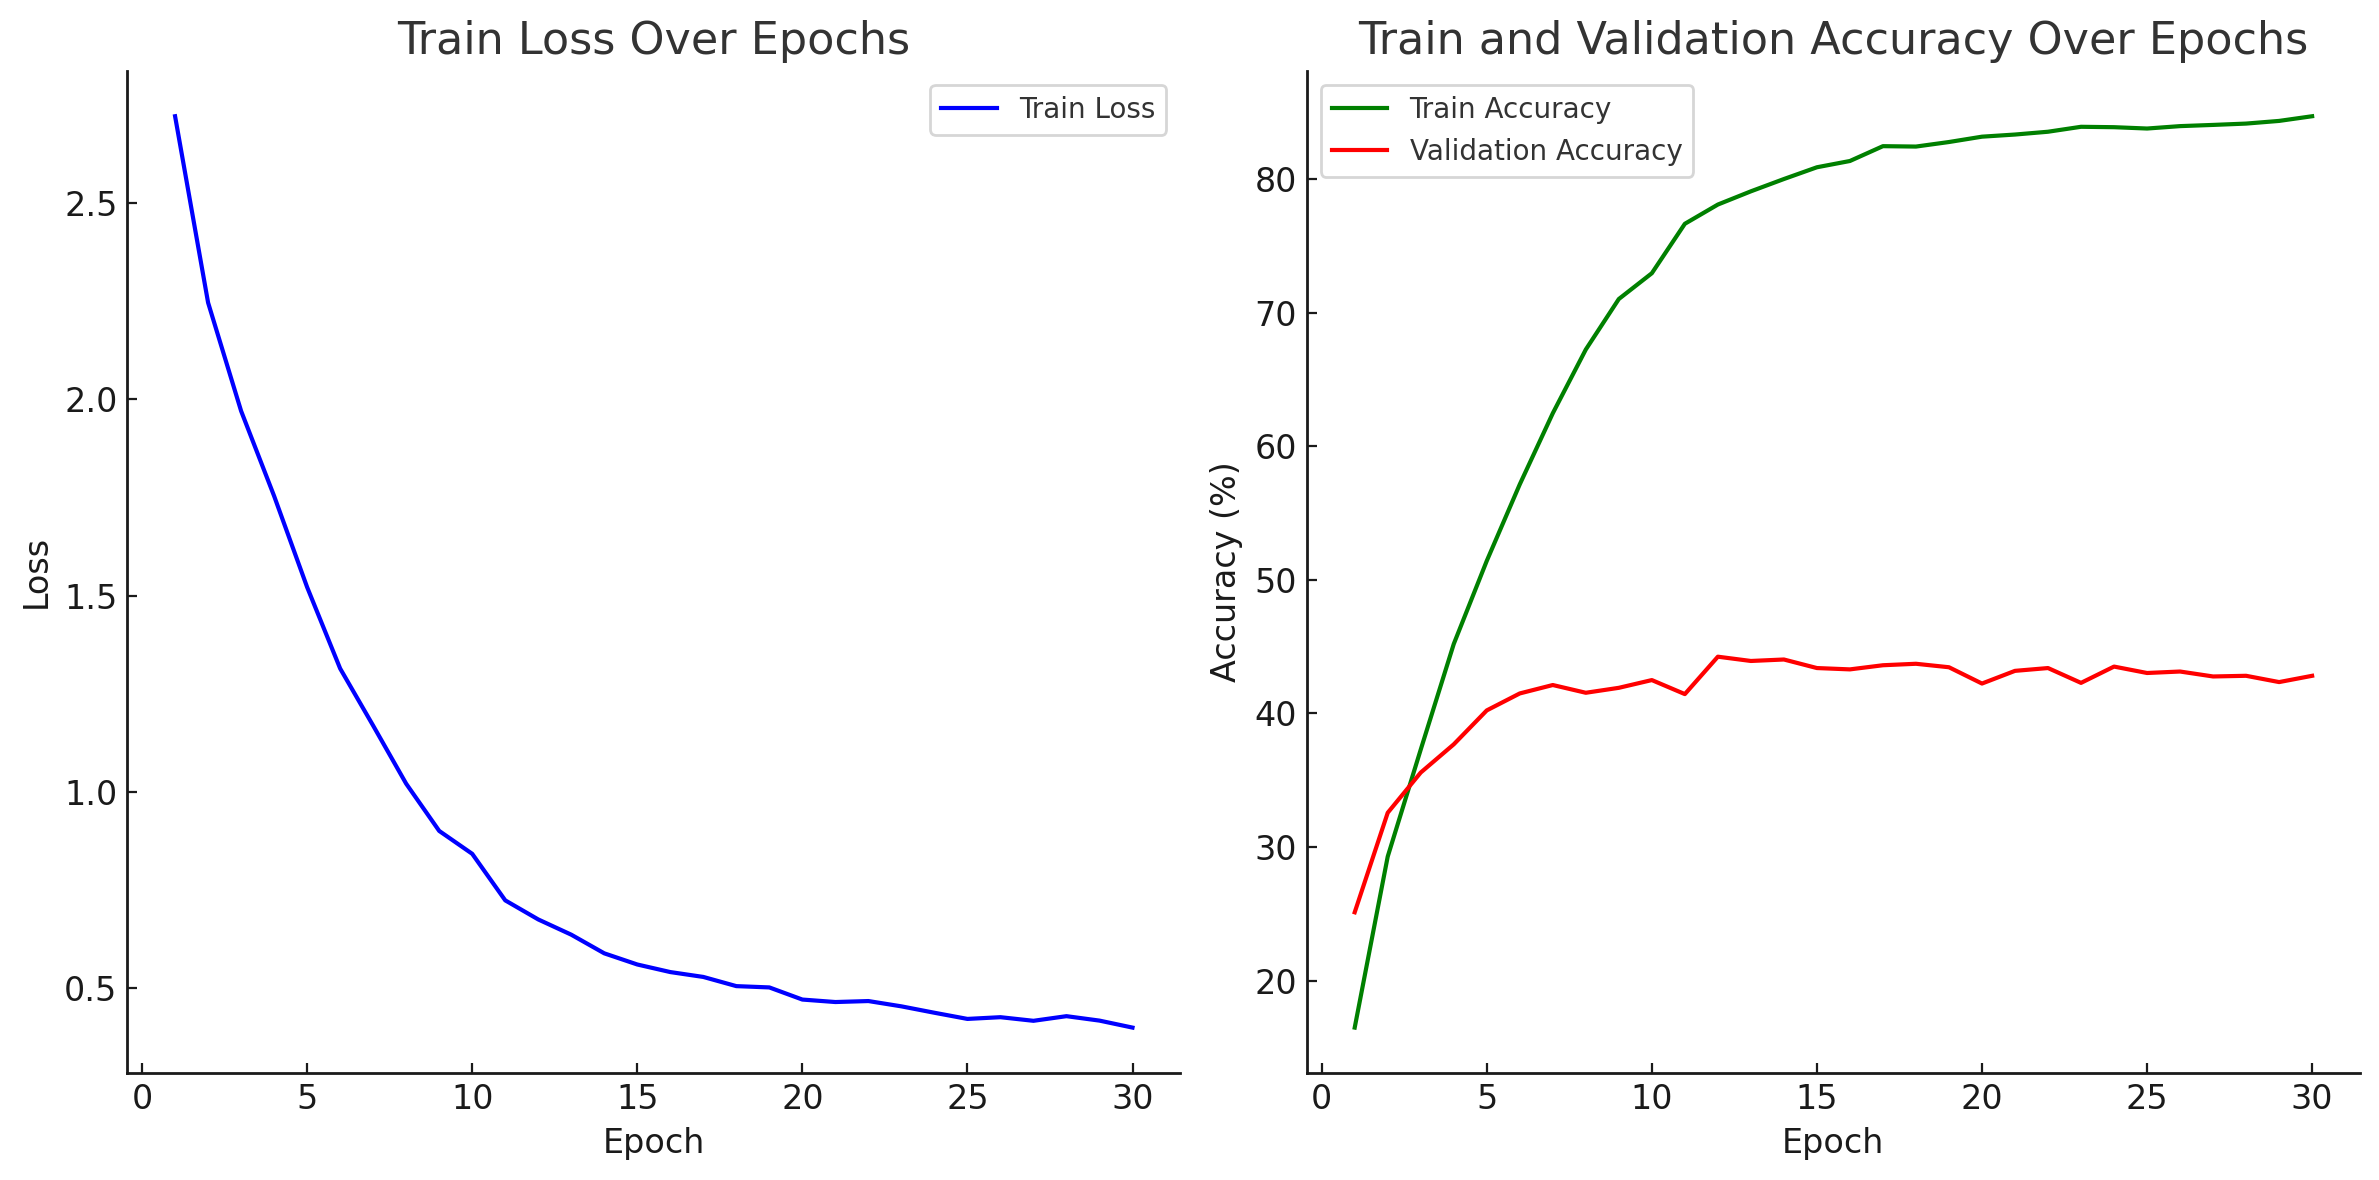
\includegraphics[width =\textwidth]{pics/Train_Loss_and_Accuracy.png}
\caption{Train Loss and Accuracy}
\label{fig:Train_Loss_and_Accuracy}
\end{figure}

As we can see,on the left graph, the train loss decreases steadily over 30 epochs, indicating that the model is learning and improving its fit to the training data. On the right graph, the training accuracy shows continuous improvement, reaching close to 80\%. However, the validation accuracy plateaus at around 40\%, showing a significant gap between training and validation performance. This suggests the model is over-fitting—performing well on the training data but struggling to generalize to unseen data. 

To assess the accuracy of a classification model which is imbalanced,the  confusion matrix provides a detailed breakdown of how well the model is performing by showing the correct and incorrect predictions in a matrix format. (Fig.~\ref{fig:Confusion_Matrix_of_CNN})

\begin{figure}[htbp]
\centering
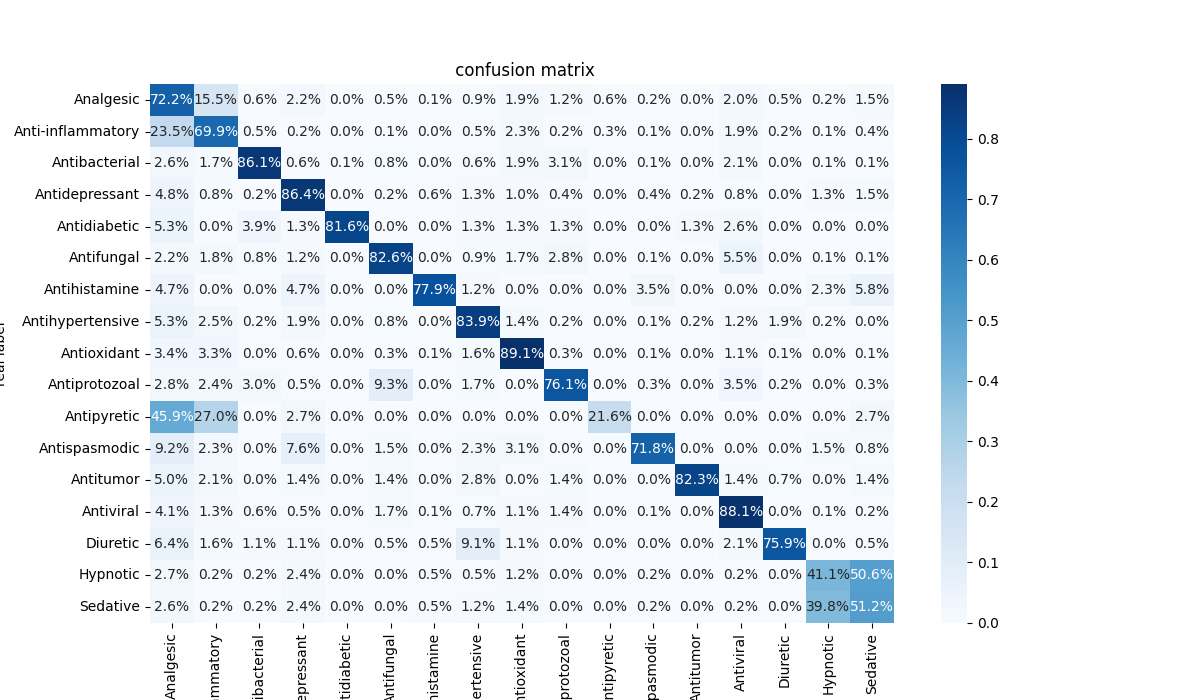
\includegraphics[width =\textwidth]{pics/Confusion_Matrix_of_CNN.png}
\caption{Confusion Matrix of CNN}
\label{fig:Confusion_Matrix_of_CNN}
\end{figure}

The heatmap reveals a concentration of high values along the diagonal, indicating that the model generally performs well in most categories.
Some classes, particularly those with overlapping effects (e.g., analgesics and anti-inflammatory drugs, hypnotics and sedatives), exhibit higher off-diagonal values, suggesting areas where further feature extraction or dataset refinement could improve performance. However, there is room for improvement in classes with overlapping effects or shared characteristics, such as hypnotics, sedatives, and antipyretics. Addressing these issues may involve incorporating additional features, refining the dataset, or using advanced techniques like hierarchical classification to handle closely related categories more effectively.

For the purpose of improving the CNN model and addressing the issue of over-fitting observed in the training results, we believe the following strategies can be employed. Data augmentation can increase the diversity of the training dataset, helping the model generalize better. Regularization techniques, such as dropout and L2 regularization, can reduce reliance on specific features and prevent over-fitting. Simplifying the model by reducing its complexity or adding batch normalization layers can also improve generalization. Leveraging pretrained models through transfer learning is another effective approach, especially for smaller datasets. Additionally, using early stopping, adjusting the learning rate, and performing hyper-parameter tuning can optimize training and prevent over-fitting. 
\section{VGG-16}

\subsection{Model Architecture}
VGG-16 is a deep convolutional neural network consisting of 16 layers, including 13 convolutional layers and 3 fully connected layers. The model uses small 3x3 convolutional filters stacked in layers, followed by max-pooling layers to reduce spatial dimensions.(as shown fig\ref{fig:VGG_pic1}) This architecture allows for high-level feature extraction, making it suitable for complex image classification tasks. However, its depth and large number of parameters make it computationally intensive, which may not be ideal for smaller datasets or tasks requiring lightweight models.

\begin{figure}[htbp]
    \centering
    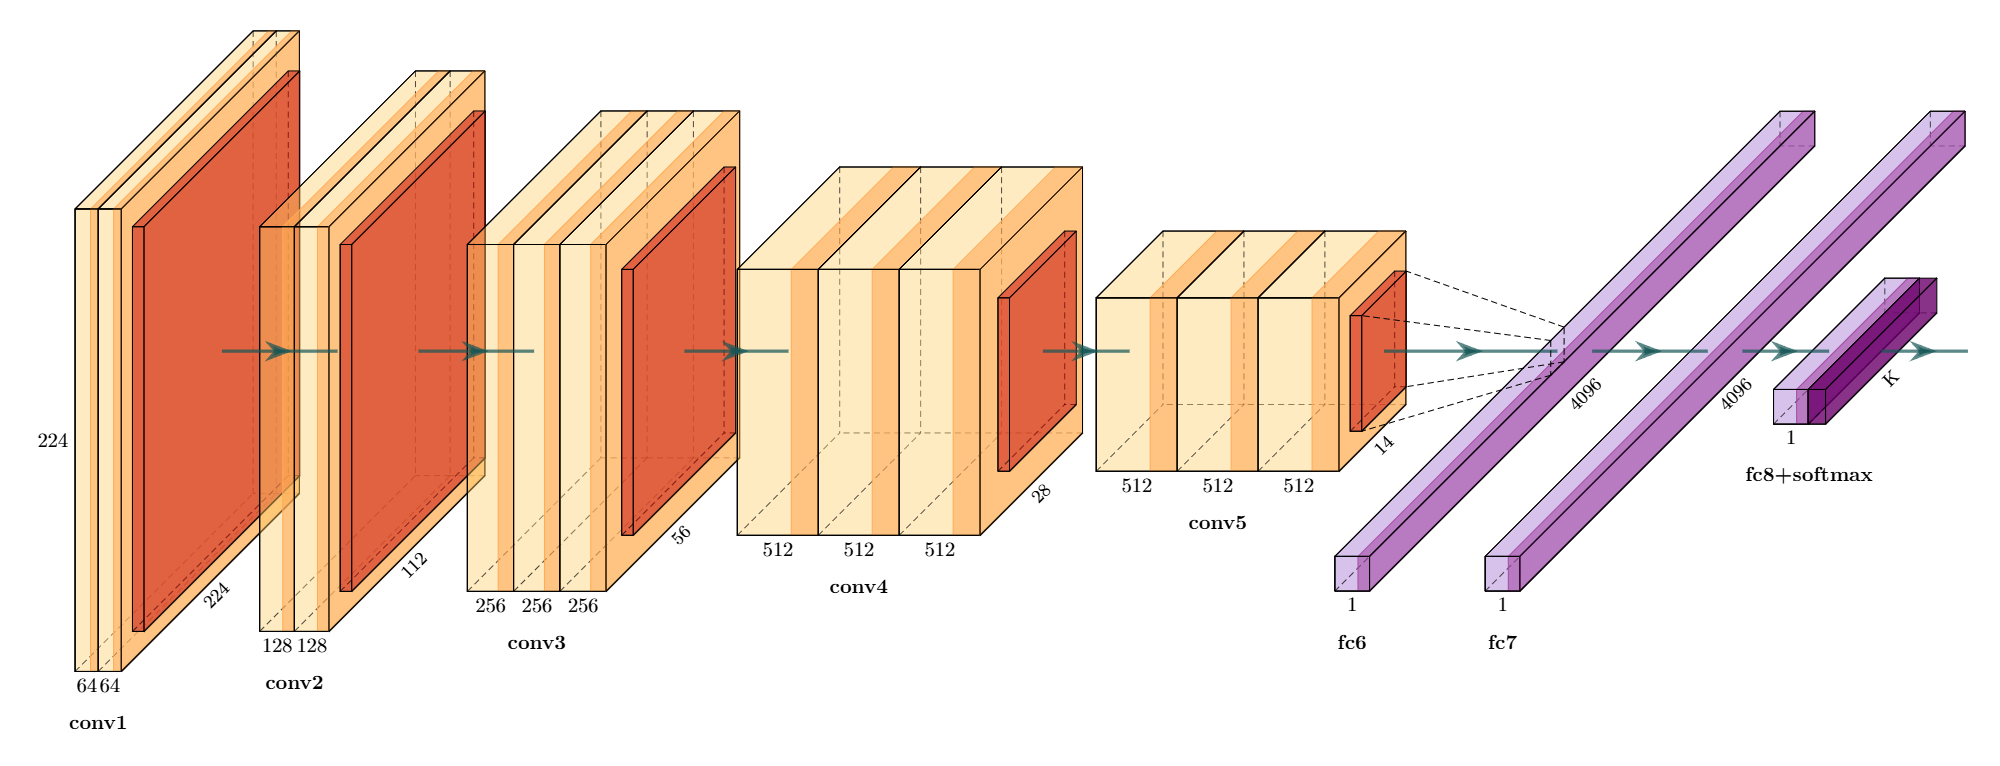
\includegraphics[width=\textwidth]{pics/VGG16_pic1.png}
    \caption{VGG-16 Train and Validation Accuracy over Epochs}
    \label{fig:VGG_pic1}
\end{figure}
We attempted to use the VGG-16 model for optimizing the classification of small drug molecules, but the results were unsatisfactory. As shown in Figure~\ref{fig:VGG_pic2}, the training loss remains consistently high (around 2.5) with minimal fluctuation over 30 epochs, indicating that the model fails to effectively learn from the training data. Both training and validation accuracies are low, with validation accuracy peaking at only 20\%, suggesting poor generalization and potential underfitting. This implies that the model is too simple to capture the complex patterns in the data.

\begin{figure}[htbp]
    \centering
    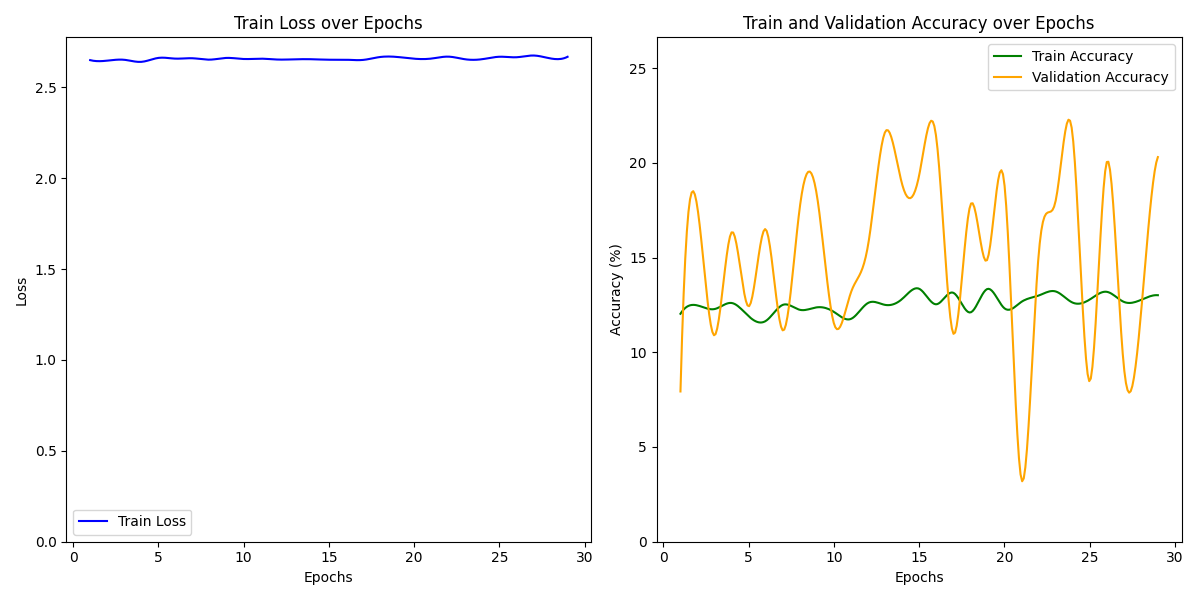
\includegraphics[width=\textwidth]{pics/VGG_pic2.png}
    \caption{VGG-16 Train and Validation Accuracy over Epochs}
    \label{fig:VGG_pic2}
\end{figure}

\subsection{Challenges and Limitations}
The poor performance of VGG-16 in our study can be attributed to several factors:
\begin{itemize}
    \item \textbf{Data Limitations}: The dataset may be too small or imbalanced, limiting the model's ability to learn meaningful patterns. Additionally, noise or incomplete feature extraction in the data could hinder performance.
    \item \textbf{Model Suitability}: VGG-16, designed for large-scale image datasets, may not be well-suited for the structural complexity of chemical compounds. Its deep architecture requires substantial computational resources and may struggle with smaller datasets.
    \item \textbf{Training Issues}: The model may require more training epochs or better hyperparameter tuning to improve convergence. The high training loss and low accuracy suggest underfitting, indicating that the model is too simple to capture the data's complexity.
\end{itemize}

\subsection{Comparison with Traditional CNN}
Compared to traditional CNNs, VGG-16 offers a more sophisticated and deeper architecture, enabling high-level feature abstraction for complex tasks. However, this comes at the cost of increased computational demands. Traditional CNNs, with their simpler and shallower designs, are more efficient and better suited for smaller datasets or less complex tasks. This highlights the trade-off between model depth and computational efficiency in deep learning applications.

To address these challenges, future work will focus on expanding the dataset, improving data quality, and exploring alternative architectures better suited for compound classification tasks. Additionally, hyperparameter optimization and regularization techniques will be employed to enhance model performance and generalization.
\section{Conclusion}

In this study, we explored the application of machine learning techniques, particularly Convolutional Neural Networks (CNNs) and VGG-16, to enhance the drug discovery process by analyzing 2D chemical compound data. Our research demonstrated that CNNs are effective in processing 2D molecular representations, significantly improving the accuracy of compound classification compared to traditional methods. However, we encountered challenges such as overfitting, where the model performed well on training data but struggled to generalize to unseen data. This issue was likely due to the limited dataset size, insufficient regularization, and the computational demands of deep architectures like VGG-16.

Despite these challenges, our findings highlight the potential of machine learning to revolutionize drug discovery by accelerating the screening process and reducing reliance on costly and time-consuming experimental methods. Future work will focus on expanding the dataset, improving data quality, and optimizing model architectures to address overfitting and enhance generalization. Techniques such as structured pruning, hyperparameter optimization, and advanced data augmentation will be employed to further refine the models.

By leveraging these advancements, we aim to develop more robust and scalable machine learning models that can significantly improve the efficiency and accuracy of drug discovery, ultimately benefiting the healthcare industry and patients worldwide.
\section{Future Work}

Our future efforts will focus on two key areas:

\subsection{Model Optimization}
We will optimize the VGG-16 architecture through structured pruning, removing redundant neurons and connections to improve efficiency and generalization. Additionally, we will explore hybrid models combining CNNs with graph neural networks (GNNs) or recurrent neural networks (RNNs) to better capture spatial and temporal dependencies in molecular data.

\subsection{Overfitting Mitigation}
To address overfitting, we will implement advanced hyperparameter optimization techniques, such as Bayesian optimization, to fine-tune learning rates, batch sizes, and regularization. Enhanced data augmentation techniques, including rotation and scaling of 3D molecular structures, will also be employed to increase dataset diversity and improve model robustness.

These improvements aim to enhance the efficiency, accuracy, and scalability of our models, advancing drug discovery and benefiting the healthcare industry.\section{GitHub Repository}

All our code and data can be found in our GitHub repository: \url{https://github.com/Fully-ripe-mango/AIGroup}

if you want to know the details of our work,or you want to test our model,please feel free to visit our repository.
\section{Contributions}

\noindent \textbf{Hanmo Shi:}
\begin{itemize}
    \item Project background and research introduction
    \item Defects and causes of the VGG-16 model
    \item Reasons for overfitting in CNN models
    \item Project summary
\end{itemize}

\noindent \textbf{Qixuan Wang:}
\begin{itemize}
    \item Construction of the final paper framework
    \item Some data visualization work
\end{itemize}

\noindent \textbf{Yingying He:}
\begin{itemize}
    \item Writing part of the thesis content
    \item Literature review
    \item PowerPoint making
\end{itemize}
\noindent \textbf{Yuxiang Tian:}
\begin{itemize}
    \item Model construction and training
    \item Thesis outline development,formatting revision and integration,Content revision
    \item Writing part of the thesis content
    \item Partial visualization (Figures  \ref{fig:How to get data},\ref{fig:Thumbnails_of_Our_CNN_model},\ref{fig:Confusion_Matrix_of_CNN},\ref{fig:VGG_pic1},\ref{fig:VGG_pic2})
    \item GitHub repository management
\end{itemize}
\printbibliography % 生成参考文献列表
\end{document}